
\chapter{Methods}
In this chapter the experimental methods and results of simulations are presented. 
In the first part the main technique used in this study is introduced. Time correlated single photon counting (TCSPC) is the most important technique in fluorescence analysis to extract the time constants of sample kinetics. In the presented study it has been proposed for VUV excitation (see chapter 7) and $\gamma$ excitation (see chapter 8).
In particular the excitation and detection time spread is the crucial parameter to deliver good performance in terms of confidence interval on measured parameters.
Moreover, a maximum likelihood method to fit the data is here presented, as well as the main sources of error leading to uncertainties in the determination of rise and decay constants.
The rise time extracted from the fit is the result of different processes happening in the crystal volume: energy deposition, electron hole relaxation, photon production (scintillation and Cerenkov), transportation to the photo detector. In order to define the relative weight of this ensemble of processes a simulation study based on Geant4 is presented.

\section{Time Correlated Single Photon couting}

The time correlated single photon counting (TCSPC) technique makes use of low-level signals at high repetition rate, with the probability of detecting on photon in one repetition period being very low \cite{Becker2005}.
It is then sufficient, to determine the time profile of the sample, to measure the time of arrival of single photons and build up a histogram of the photon times, as shown in figure \ref{fig:tcspc}.
The most common method to perform this measurement is a start-stop setup: some sort of trigger, correlated with the beginning of the excitation process in the sample (start), is measured in coincidence with a stop signal given by the arrival of the optical photon emitted by the sample.
\begin{figure}[htbp]
\begin{center}
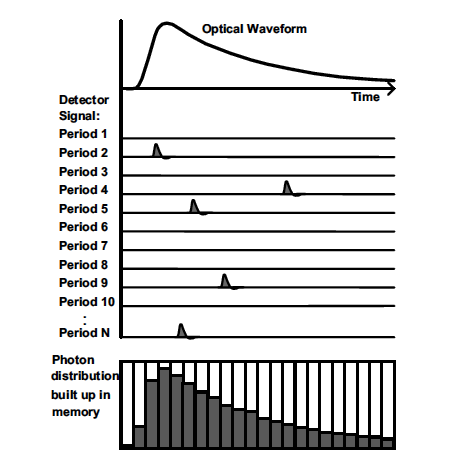
\includegraphics[width=9cm]{../Pictures/Chapter_6/tcspc.png}
\end{center}
\caption[TCSPC technique]{Principles of time correlated single photon counting (TCSPC)}
\label{fig:tcspc}
\end{figure}

Thus the main components of a TCPSC system are
\begin{itemize}
\item an excitation system for the sample with an extracted trigger
\item a fluorescent sample with a characteristic periodic light emission
\item a detection system able to extract the time stamps of the arriving single photons.
\end{itemize}
The effective resolution of a TCSPC experiment is characterized by its instrument response function (IRF). The IRF is the result of the pulse shape of the light source used, the temporal dispersion in the optical system, the transit time spread in the detector, and the timing jitter in the recording electronics.
The main sources of error and incertitude on the measured curve are presented in this chapter and can be roughly categorized as:
\begin{itemize}
\item the time structure of the excitation
\item the single photon time resolution of the detection system
\item the rate of arrival of optical photons at the stop detector
\item the long accumulation times
\end{itemize}

\subsection{Excitation}
In an ideal TCSPC experiment, the excitation system has a very narrow distribution in time. That is, the spread of the single particles determining the excitation of the sample is negligible with respect to the time scale of the processes under study.
A variety of high time resolution sources are available for TCSPC. In classical fluorescence studies laser sources (or laser-driven) sources are used and allow for the study of sub-ps dynamics: mode-locked Argon or Nd:YAG lasers, synchronously pumped dye lasers, or Ti:Sapphire lasers.
For the time scales that characterize electron hole thermalization, thus signal formation, thus rise time in scintillating crystals, it is necessary to make use of a ps resolved system.

The main limitation though, comes from the excitation energy of the system, since the level of excitation is crucial in determining the physical processes that concur to give a non zero rise time. 
As was shown in previous chapter, the multi scattering processes that lead electrons and holes below the ionization threshold, and thus to the accuracy limit of Monte-Carlo simulations, happen on time scales which are an order of magnitude smaller than thermalization stage. 
This means that in terms of physical processes not much is added to the study by raising the excitation energy above 10 time the band gap of the sample.
Two different phenomena though introduce a non-negligible contribution to the time spread of the rise if the signal collected.

The first one is the appearance of Cerenkov photons, above the threshold for the specific materials. Thresholds for Cerenkov effect in heavy scintillating crystals have been briefly summarized in chapter 2.
These photons, although in a limited number, are concentrated in the very first portion of the time profile. This results in a modification of the rise time towards longer values.
In order to asses the relative impact of these effects, the samples were measured in different conditions of excitation: at a high harmonics generation facility with a 36 eV VUV radiation and in a experimental bench with a 511 keV radiation.

A second prominent source of smearing in time profiles is the travel of photons inside crystalline samples \cite{Derenzo2000}. Indeed, depending on the type of coupling to the photo detector, photo extraction can be favoured or disfavoured at different angles. Opening this extraction cone accounts for different time profiles: a Teflon diffusive wrapping or coating for example, gives longer rise times. From the point of view of the excitation energy, though, an important difference can be found at 36 eV or 511 keV. In the first case the excitation is only on the surface, since the range of VUV photons in a heavy scintillator is of the order of a few hundred nano meters.
In the case of excitation at higher energy, on the other hand, photons may travel longer distances in the lattice, and photons produced in the deep volume of the sample need to be coupled out.

\subsection{Detection}

Once the sample has been excited, photons are coupled out to the stop detector. Typically PMTs, MCP-PMTs or single cell APD in Geiger mode are the preferred detectors for their timing characteristics. The crucial parameter in this case is Single Photon Time Resolution (SPTR) for Silicon detectors or Transit Time Spread (TTS) for vacuum detectors.
It is clear that in order to extract the most accurate value for the time constants of the samples measured, one should keep the incertitude component due to the detector as low as possible. In this case it is customary to make use of detectors optimized for single photon detection that is with low or no energy resolution and very rapid response.
For the study presented MCP-PMTs have been mainly used, since in principle they guarantee the best performance when considering acquisition rates and time resolution.
As will be clear in the next chapters, this prerogative of MCPs becomes less and less attractive as the energy of the excitation grows, since it is necessary to cope with non-negligible backgrounds due to the high active area.
Nevertheless, given the time scale considered in this study, a response of less than 100 ps should be available in order to extract the parameters with a minimum accuracy. As will be presented in the next chapters the photo detectors chosen for this study satisfy this requirement.
Many stop detectors, and this is the case of the MCPs used in the next analysis, present an important amount of time walk, and often require appropriate corrections.
Time walk arises when synchronous signals have different amplitudes. Time pick up methods based on threshold crossing may extract different time stamps and thus introduce a non negligible jitter.

\subsection{Stop rate and bias}
When considering the geometry of the experiment, another parameter becomes crucial: the stop rate at the detector.
As explained before two opposite effects tend to counteract; ideally we should keep the count rate as high as possible to have reasonable accumulation times, but the increasing of the bias fraction of counts modify the profile measured.
Two techniques will be used in this study, employing a conventional TDC and a multi-hit TDC.
A conventional TDC can only digitize the arrival time of the first stop signal. Therefore events that have more than one stop pulse will bias the data set, since the later pulses will not be measured with the same probability. This will be the case of the acquisition setup presented in chapter 7.
If we define the probability P that m photons are detected after a single excitation, the Poisson distribution gives
\begin{equation}
P(m;\epsilon) = \epsilon ^{m} e ^{-\epsilon} / m!
\end{equation}
and $\epsilon$ is the average number of stop per excitation.
The probability to have an unbiased event is
\begin{equation}
Event_{unbias} = U = P(1;\epsilon) = \epsilon e ^{-\epsilon}
\end{equation}
and the probability to have a biased event is, assuming $\epsilon << 1$
\begin{equation}
Event_{bias} = B = \sum _{m = 2} ^{\infty} P(m;\epsilon) \sim \epsilon ^{2} e ^{-\epsilon} / 2
\end{equation}
The ratio of biased to unbiased event is given by
\begin{equation}
B/U \sim \epsilon / 2
\end{equation}
The factor $\epsilon$ depends on the combined effect of the geometry of the system, the light yield of the crystal, the quantum efficiency of the detector. In order to improve the ratio, it is thus necessary to lower the rate at the detector by modifying the position accordingly, at the expense of reduced data collection rates.

On the other hand, in chapter 8 a multi-hit approach will be proposed, that is capable of measuring the arrival of n stop pulses per start pulse. In this configuration the data acquisition rate can be increased, as the probability is:
\begin{equation}
Event_{unbias} = \sum _{m = 1}^{n}mP(m;e) = \sum _{m = 1}^{n} \frac{\epsilon ^{m}e^{-\epsilon}}{(m-1)!}
\end{equation}
With a higher photon flux and events with more than one stop signal, it is possible that the difference in the arrival time of two of such pulses is less than the dead time of the detector. In this case only the first of the two photons will be registered. We can define the parameter d as the ratio between the dead time of the system and the decay time of the sample, or $d = DT/\tau _{d}$.
Figure \ref{fig:bias_decay} shows the fraction of biased measurements as a function of $\epsilon$ simulated for different values of d.
In the case of most of the samples measured in this study, the dead time of the detection system is usually $\sim$ 1 ns. The decay time is usually $<$ 100 ns. Therefore the value of d is $\sim$ 0.3. From the plot we can then conclude that for $\epsilon = 0.2 $ the bias ratio is less than 1$\%$, and this will be the value tolerated for the data analysis.
\begin{figure}[htbp]
\begin{center}
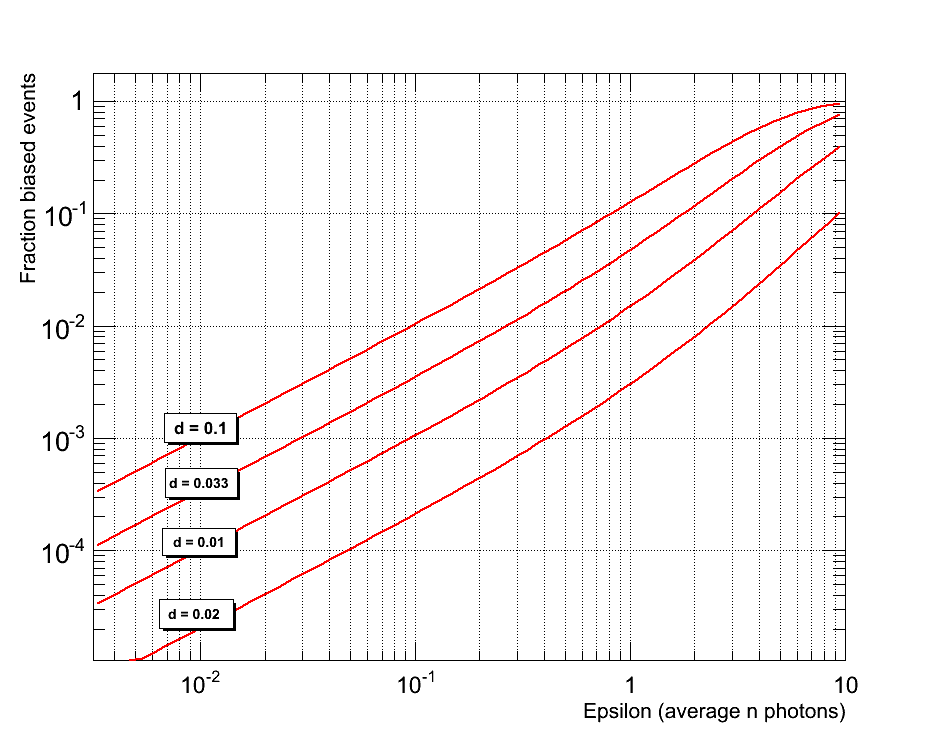
\includegraphics[width=10cm]{../Pictures/Chapter_6/bias_function.png}
\end{center}
\caption[Bias fraction in multi hit TCSPC]{Evolution of the bias fraction as a function of the count rate for a multi-hit TCSPC. The variation is shown for different values of $d = DT/\tau _{d}$.}
\label{fig:bias_decay}
\end{figure}
Given the number of photons in the first time bins and the integration, the rise time is less prone to bias given by high count rates. The toy model used before to determine the bias ratio was extended to produce simulated pulses. This pulses were later fit to extract the rise time. The result is shown in figure \ref{fig:bias_rise} for different values of $\epsilon$ and $\tau _{r} = 100$ ps.
It is clear that the effect of high count rates is an increase of the bias, but even for very high values the rise time is underestimated by less than 10 ps, which is far less than the confidence interval on the parameter given by the likelihood fit.
\begin{figure}[htbp]
\begin{center}
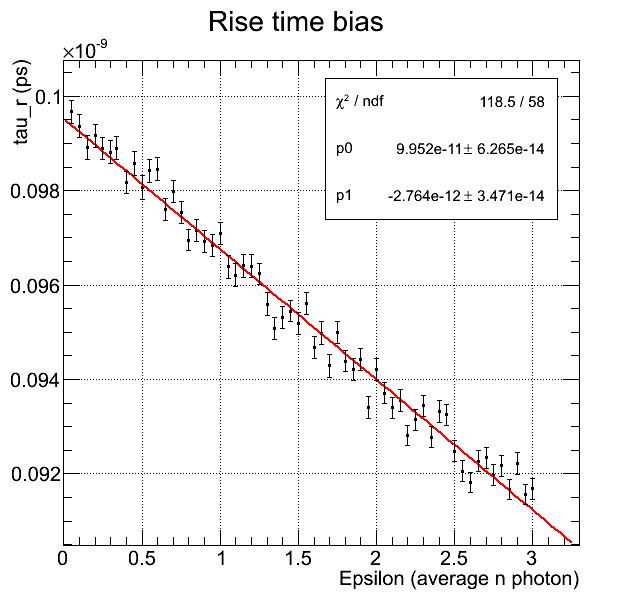
\includegraphics[width=10cm]{../Pictures/Chapter_6/bias_rise.png}
\end{center}
\caption[Rise time bias in multi hit TCSPC]{Evolution of the fit rise time as a function of the count rate for a multi-hit TCSPC, given a original value of 100 ps.}
\label{fig:bias_rise}
\end{figure}

\section{Data analysis techniques}
In order to analyse the start stop data collected, a classical fitting approach was used, based on maximum likelihood principles.
With respect to this statistical and systematic contributions to the error were estimated, based on the previous discussion.
In particular the iterative re convolution approach has been used, being the most powerful and widespread in the field of fluorescence lifetime measurements.

\subsection{Iterative re-convolution}
In time correlated single photon counting experiments the problem at hand is, statistically speaking ,to estimate one or more parameters (the lifetimes) from a data set.

The maximum likelihood method is considered to be the most powerful method of parameter estimation.
Consider $n$ independents observation (counts in this case) c$_{1}$, ... , c$_{n}$ and a vector of parameters \textbf{$\theta$} = $(\theta _{1},...\theta _{m})$. If the probability of having the observation i is $p(c_{i}|\theta)$, the likelihood function is
\begin{equation}
L(c_{1},...c_{n}|\theta) = \prod _{i = 1} ^{n} p(c_{i}|\theta) 
\end{equation}
The Maximum Likelihood method provides then an estimate of the true value of the parameters as the vector \textbf{$\theta$} that maximizes the likelihood function.
In the case of time correlated single photon counting it is natural to assume that the observed counts $c_{i}$ follow a Poisson distribution
\begin{equation}
p(c_{i}|\theta) = \exp{ \left( -<c_{i}>\right) }\frac{<c_{i}>^{c_{i}}}{c_{i}!}
\end{equation}
where $<c_{i}>$ is the expected value of the number of counts in the i-channel.
The model taken into consideration gives this expected value: in this case we can make use of the equations obtained in chapter 3. The pdf for the time stamps is given by
\begin{equation}
p_{t_{n}}(t|\theta) = A \cdot \sum _{i} \frac{S_{i}}{\tau _{d,i} - \tau _{r,i}} \cdot \left[ a_{\tau _{d, i}}(t|\theta) - a_{\tau _{r,i}}(t|\theta)\right]
\end{equation}
where 
\begin{eqnarray}
a _{\tau}(t|\theta) &=& \frac{1}{2} \exp{\left(\frac{\sigma _{SPTR} ^{2} - 2\tau t +2\tau \theta + 2\tau t_{TT}}{2\tau ^{2}}\right)} \\
&& \cdot \left[ erf\left( \frac{t-\theta -t_{TT} - \frac{\sigma ^{2}_{SPTR}}{\tau}}{\sigma _{SPTR}\sqrt{2}} \right) + erf \left( \frac{t_{TT}+\frac{\sigma ^{2} _{SPTR}}{\tau}}{\sigma _{SPTR}\sqrt{2}} \right) \right]
\end{eqnarray}
Thus the expected number of counts for the i-channel is
\begin{equation}
<c_{i}> = \int _{(i-1)\Delta} ^{i\Delta} p_{t_{n}}(t|\theta)dt + b_{i} = g _{i}(\theta)
\end{equation}
where $\Delta$ is the time channel width and $b_{i}$ accounts for the average number of dark counts in the channel i.
The vector of parameters \textbf{$\theta$} is given by the lifetimes $\tau _{i}$, the relative intensities $S_{i}$ and a zero time shift $\delta$.
It is customary to determine the best estimate for \textbf{$\theta$} by minimizing the function $-ln(L)$ since the log-likelihood function attains its maximum for the same value as the likelihood function.
In the specific case the function to minimize is
\begin{equation}
-\log {L} = - \prod _{i=1}^{n} \exp {-g_{i}} \frac{g_{i}^{c_i}}{c_{i}!} = \sum _{i=1}^{n} -g_{i} + c_{i}\log {g_{i}} - \log {c_{i}!}
\end{equation}
which is equivalent to minimizing the Poisson deviance\cite{Bajzer1991}
\begin{equation}
f = \sum _{i=1}^{n} -g_{i} + c_{i}ln(g_{i})
\end{equation}
The standard function minimized in standard fluorescence analysis is usually the $\chi ^{2}$ defined as
\begin{equation}
\chi ^{2} = \sum _{i=1}^{n} \frac{\left[ c_{i} - g_{i}(\theta) \right] ^{2}}{c_{i}}
\end{equation}
or, in the modified least square method\cite{Bajzer1991}
\begin{equation}
\chi _{m}^{2} = \sum _{i=1}^{n} \frac{\left[ c_{i} - g_{i}(\theta) \right] ^{2}}{g_{i}}
\end{equation}
When the number of counts is large they are numerically very close, since the Poisson distribution can be approximated by the Gaussian. Nevertheless in the data analysis the maximum likelihood estimator will be used, since it is preferable the more the low-count region of the decay influences the estimated parameters\cite{Bajzer1991}. 

\subsection{Estimation of confidence intervals}
As we discussed the main source of bias in the measurement comes from the count rate at the stop detector. The statistical error associate with the extracted parameters can be determined from the likelihood fit procedure.
In order to determine the confidence interval on the parameters it is necessary to consider the rise time and the decay time and the influence of collected statistics.
The fit procedure has been presented in the last section and it consists in the minimization of the function $-\log{L}$.
The software used for minimization is Matlab.

We consider here only the case for one decay component. It is usually enough to consider only the first component, especially if it is significantly longer than the rise time constant. This is the case for most of the samples measured: as an example the LSO Cerium doped compounds present a rise time in VUV excitation of the order of $\sim$ 50 ps and a decay time of the order of $\sim$ 40 ns.
In order to quantify the effect of mutual variation of fit parameters, a simple toy model was used with the shape described above. The analysis was then performed over the samples measured for parameters estimation.
The toy model used presents in this case a rise time of 36 ps and a decay time of 33 ns. 

For what concerns the confidence level on the parameters extracted from the fit, we profiled the two dimensional likelihood over the parameters optimized, that is rise time and decay time, as shown in figure \ref{fig:likelihood} for different number of counts collected for the rise time.
In this case a binned likelihood approach requires a determination of a confidence interval based on an asymmetric likelihood.
At the best fit point the function to minimize  $-2\ln{L}$, tends to a chi-squared distribution for (n-2) degrees of freedom. In this case it is customary to define a confidence level the interval ($min_{L}$, $min_{L}+\frac{1}{2}$) since in the limit of normally distributed data for large counts it translates to a 95$\%$ confidence level. In this case the likelihood is close to this approximation, therefore this convention will be used for confidence intervals.
In figure \ref{fig:likelihood} the likelihood function marginalized for the rise time is shown, for different number of counts. The interval ($min_{L}$, $min_{L}+\frac{1}{2}$) is shown on the picture as well as the derived confidence interval. The same methodology will be used to extract the uncertainty on the decay time.
\begin{figure}[htbp]
\begin{center}
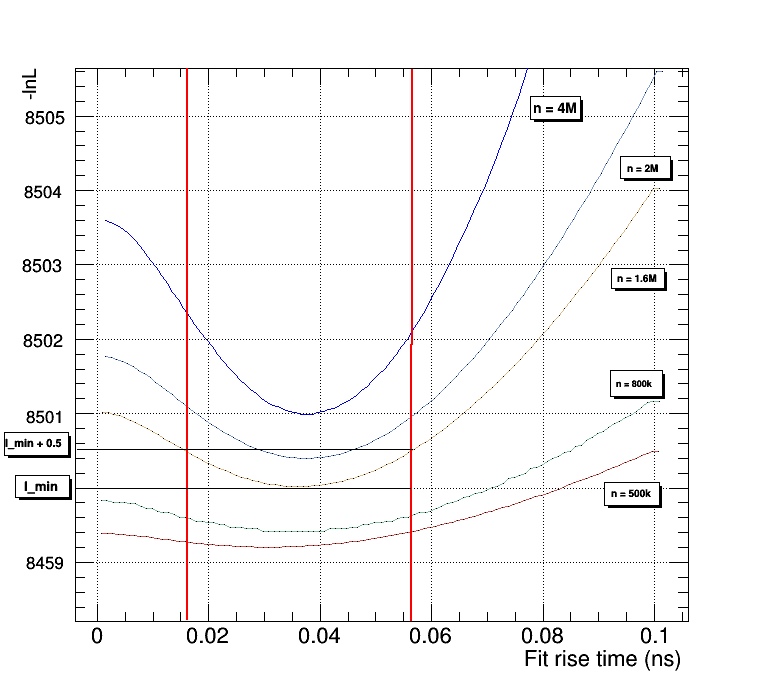
\includegraphics[width=10cm]{../Pictures/Chapter_6/error_rise.png}
\end{center}
\caption[Influence of statistics on likelihhod]{The statistics collected is varied from 100000 to 4000000 and the influence on the likelihood for extracted rise time is shown.}
\label{fig:likelihood}
\end{figure}

\section{Simulations}

As already stated, Geant4 allows for a partial characterization of the signal formation in heavy scintillating crystals.
In particular we can formalize the processes leading to the collection of optical photons at the detector in four steps:
\begin{itemize}
\item energy deposition
\item electron hole recombination
\item emission of scintillation photons
\item transport of optical photons
\end{itemize}
A fourth process to be considered is the production of Cerenkov photons, which leads at these energies to negligible energy depositions, but has a non negligible impact on timing.

\subsection{Energy deposition and recombination}
The energy deposition phase has a small impact on the signal formation above the ionization threshold in the case of scintillation. Indeed, as seen in \cite{Lecoq2006}, processes leading to the production of electron hole pairs at the ionization level occur at a time scale of about 1 pico second. This entails that oscillations in the energy deposition time lead to negligible influences on the formation of the signal. As an example we can consider the interaction of a 511 keV $\gamma$ in a LSO crystal. In figure \ref{fig:energy_dep} the energy deposition profile for electrons at the cut value is shown. In this case the cut value is 250 eV, that is the lowest value for G4Penelope low energy libraries. At this cut value, the tracking of the particle is interrupted, and the electrons are not able to produce any further ionization or other interaction.  
\begin{figure}[htbp]
\begin{center}
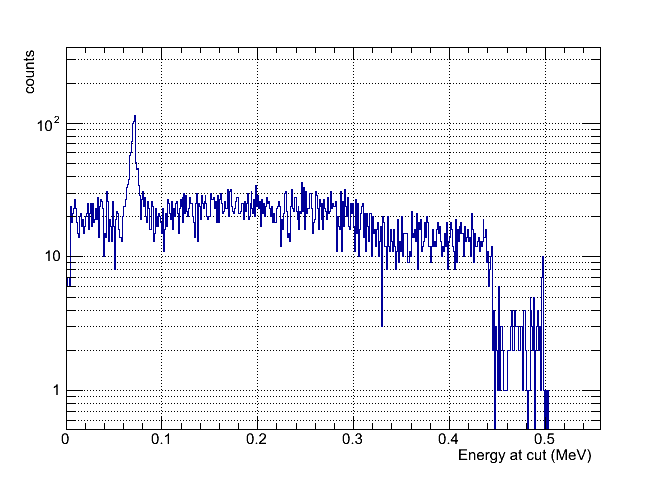
\includegraphics[width=10cm]{../Pictures/Chapter_6/energy_und_thr.png}
\end{center}
\caption[Energy deposition at 250 eV]{Energy deposition at the 250 eV threshold (G4Penelope libraries) for LSO. The interacting $\gamma$ has an energy of 511 KeV.}
\label{fig:energy_dep}
\end{figure}

If we analyse at the tracking step the time at the energy deposition, and thus at the cut value, we find substantial confirmation for the marginal impact of this stage for the rise time. Indeed in figure \ref{fig:energy_dep_time} the RMS on this deposition time is $\sim$ 2 ps.
\begin{figure}[htbp]
\begin{center}
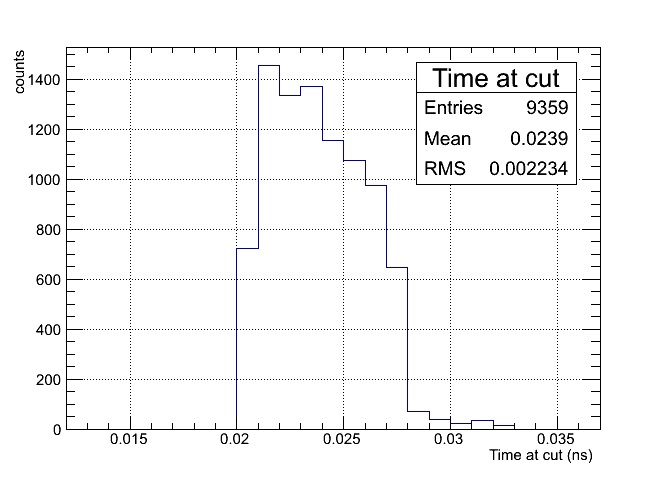
\includegraphics[width=10cm]{../Pictures/Chapter_6/time_und_thr.png}
\end{center}
\caption[Time of deposition at 250 eV]{Energy deposition time at the 250 eV threshold (G4Penelope libraries) for LSO. The interacting $\gamma$ has an energy of 511 KeV.}
\label{fig:energy_dep_time}
\end{figure}

At this point the electron track still retains a 250 eV energy, that is more than 10 times typical band gap energies of heavy crystals. 
As already discussed in chapter 4, the core of the stochastic processes leading to non zero rise time lies at energies of $\sim$ 2 E$_{g}$, below the electron-electron scattering threshold. At this stage the time scales involved are 10$^{-14}$-10$^{-12}$ seconds, and they start to influence the time resolution importantly, since RMS transportation values and SPTR values lies typically in this range.
As a consequence simulation packages usually require the specification of a rise time, that we can define as an intrinsic quantity, defining the time scale of the thermalization processes.

\subsection{Study of optical transport}
Once photons are produced they need to be coupled out to the photo detector. The experimental condition influences both the number, the oscillations in this number (the so called energy resolution) and the collection times of the photons. 
The first parameter to consider is the aspect ratio of the sample considered. This modifies the angles at which photons arrive at boundaries, and thus the Fresnel coefficients for extraction. This has been already shown in chapter 5, in comparison with the simulation tool SLitrani.
A second element that can drastically influence the modalities of photon collection is the surface treatment. Indeed in a \textit{unified} approach we can consider a surface as made of a large number of micro facets, tilted at defined angles with respect to incident light ray. In this case the surface conditions as well as specific surface treatments, such as mechanical depolishment modify the geometrical profile of the surface.
In addition coupling media and wrappings can play a role, pretty much in the same sense: they can re couple photons which would be extracted based on a simple Fresnel approach and extract photons otherwise lost.
The combined effect of these variables is hard to be quantified, and it is usually impossible to be assessed analytically. Even in the case of Monte Carlo simulations, the uncertainties associated to the optical parameters for the materials used often prevent a precise assessment. In this situation we thus mainly rely on the measurements method presented in chapter 5 and we present result for LSO samples. Similar quantities have been extracted for the different samples measured in time resolved studies of this work.

The light output is the most delicate parameter to be considered for timing studies. As shown in chapter 4, the Fisher information, that is the statistical content of the data set in terms of time resolution, depends on the number of photons collected. For this reason the light output value plugged in the simulation was tuned on the value measured on the experimental bench. Since in this study we are not concerned with the absolute value of light yield, it has been tuned so to match the extraction efficiency shown at the end of chapter 5, with and without Teflon.

Before continuing with the discussion regarding the photons production modalities, it is interesting to quantify the influence of a simplified set of experimental conditions on the extraction times of optical photons. With respect to this we chose size ratio and wrapping condition as a benchmark.
In order to understand the influence of photon transportation we consider the production of a bunch of optical photons in different positions of LSO crystals with 2x2 mm$^{2}$ exit face and different lengths. In figure \ref{fig:refl_example} the collection time of photons is shown for a 2x2x3 mm$^{3}$ and a 2x2x20 mm$^{3}$ crystal with the optical photon source at the center of the volume. We can limit the analysis to the first two reflections, since higher order reflections are very unlikely to be coupled out and happen at longer times. 
For the 2x2x3 mm$^{3}$ crystal the two bunches happen at very close time, since the length of the crystal is reduced. In this case this peaks are very likely to be washed out by the time resolution of the system. This does not happen in the case of a longer crystal, where a significant delay shifts the reflection towards longer times.

\begin{figure}[htbp]
\begin{center}
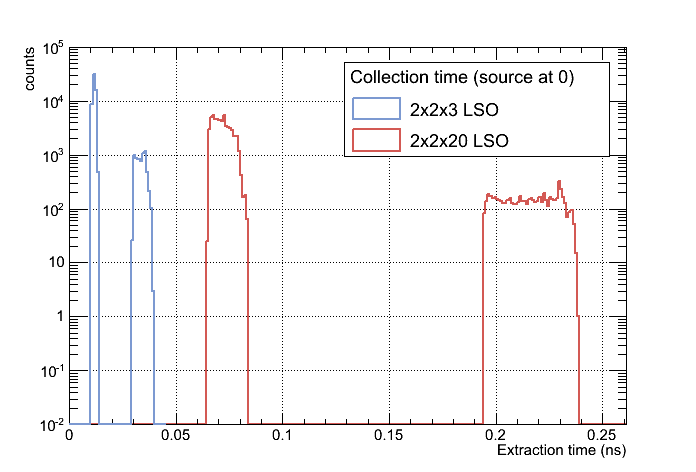
\includegraphics[width=10cm]{../Pictures/Chapter_6/reflections.png}
\end{center}
\caption[Collection time for optical source]{Collection time of photons for a 2x2x3 mm$^{3}$ and a 2x2x20 mm$^{3}$ crystal with the optical photon source at the center of the volume.}
\label{fig:refl_example}
\end{figure}
Adapting this setup to a moving source, the RMS in time of the collected photons for different crystal lengths is shown in figure \ref{fig:rms_moving} . Geometric arguments lead to consider that the RMS increases when the interaction point is closer to face opposite to the extraction one, due to the overlapping of reflection modes. The RMS is not negligible when considering the formation of the signal, since the time scale is relevant with respect to typical rise times ($\sim$ 70 ps). In the case of typical PET crystal size, 2x2x20 mm$^{3}$, the RMS for photons produced far from the detector can be as large as 10 ps.

\begin{figure}[htbp]
\begin{center}
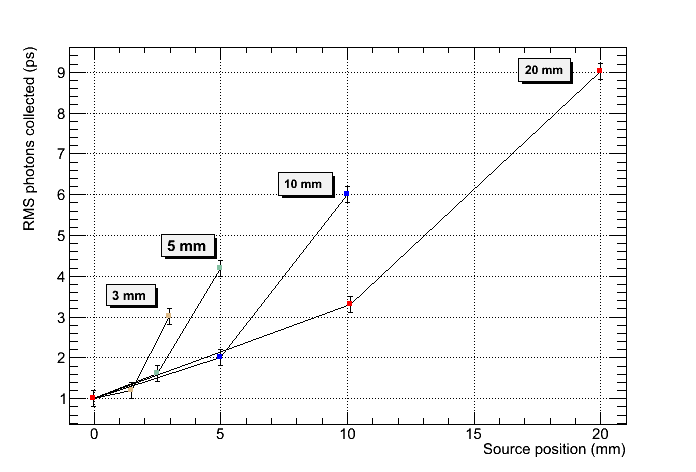
\includegraphics[width=10cm]{../Pictures/Chapter_6/rms_moving.png}
\end{center}
\caption[RMS photons for naked LSO]{RMS of the collected photons for different crystal lengths in the case of a naked LSO crystal.}
\label{fig:rms_moving}
\end{figure}

This situation is more pronounced in the case of wrapping material coupled to the crystal. In figure \ref{fig:rms_moving_wrap} the same simulation setup is adapted for Teflon wrapping. Teflon is modelled as a diffusive reflector, with absorption coefficient extracted from \cite{Kawamura1996}. The situation is qualitatively similar, but the RMS values can be as high as 20 ps. This introduces a relevant time spread in the photons collected.
The situation presented is ideal, in the sense that we consider photons interacting always in the same position of the crystal. This is not the case for PET setups, where photons may interact in different position of the crystal volume. This is not even the case for the setup presented in the time resolve study of the two last chapters. In order to interpret these results in a realistic setup, we simulated the setup of our experimental bench.

\begin{figure}[htbp]
\begin{center}
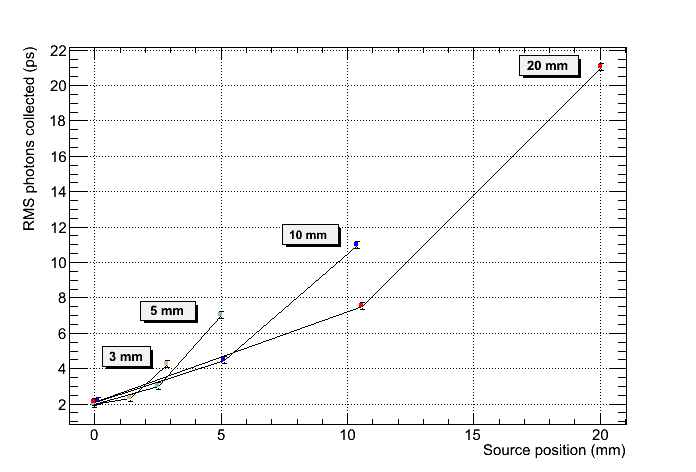
\includegraphics[width=10cm]{../Pictures/Chapter_6/rms_moving_wrap.png}
\end{center}
\caption[RMS photons for Teflon wrapped LSO]{RMS of the collected photons for different crystal lengths in the case of a Teflon wrapped LSO crystal.}
\label{fig:rms_moving_wrap}
\end{figure}

\subsection{Photon production}
We showed how different interaction points in the volume entail rather different collection  time distributions. 
In a realistic setup the depth of interaction may vary at each scintillation event, thus the final pulse shape will reflect this variation in the rising edge.
It is interesting to consider that the extraction profile of Cerenkov photons for a low energy $\gamma$ is contained in a sphere of a few hundreds nm and the production time profile can be considered prompt. This situation is quite similar to the simulation setup of the previous section, where the production of optical photons was punctual and without spread in time.
It is then interesting to compare Cerenkov photons collection times and relative RMS for different crystal dimensions, as shown in figure \ref{fig:cer_coll} for a 2x2x3 mm$^{3}$ LSO and a 2x2x20 mm$^{3}$ LSO. The simulation setup is the equivalent to the $\gamma$ detection setup presented in chapter 8, and it is a simple LSO crystal with and without Teflon wrapping with a glass sensor (PMT or SiPM).
It can be seen that for small crystals the contribution to rise time for reflected photons is very important, since it broadens the distributions of photons in the very first time slots. In the case of a longer crystal the reflection is shifted of more than 100 ps, thus influencing less the rise time measurement. In this case the RMS of photons collected may be as high as 30 ps, comprehending the production and transportation stage contributions.
%\begin{figure}[htbp]
%\begin{center}
%\includegraphics[width=10cm]{../Pictures/Chapter_6/}
%\end{center}
%\caption[Setup of the Geant4 simulation.]{Setup of the Geant4 simulation.}
%\label{fig:sim_set_gam}
%\end{figure}
\begin{figure}[htbp]
\begin{center}
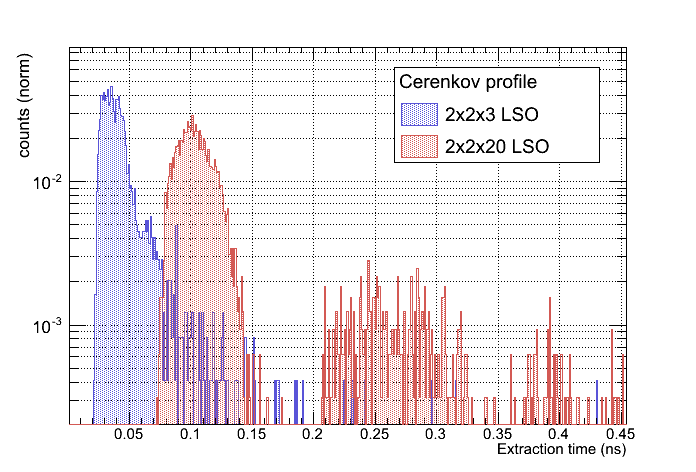
\includegraphics[width=10cm]{../Pictures/Chapter_6/cerenkov_collected.png}
\end{center}
\caption[Collection Cerenkov times for LSO naked]{Collection time of Cerenkov photons produced by a 511 KeV $\gamma$ in a LSO crystal. The cases for a 2x2x3 $mm^{3}$ and 2x2x20 $mm^{3}$ naked samples are shown.}
\label{fig:cer_coll}
\end{figure}

In the case of Teflon wrapping the RMS value increases even more, and the time collection distribution develops very long tails, as shown in figure \ref{fig:cer_tefl}.
\begin{figure}[htbp]
\begin{center}
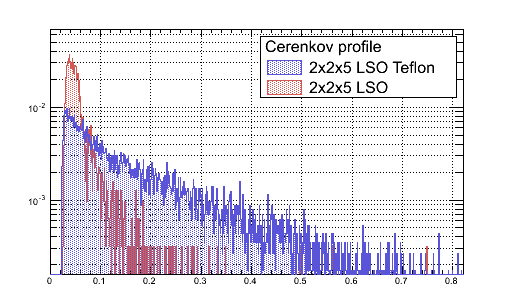
\includegraphics[width=10cm]{../Pictures/Chapter_6/cerenkov_teflon_nt.png}
\end{center}
\caption[Collection Cerenkov times for LSO Teflon wrapped]{Collection time of Cerenkov photons produced by a 511 KeV $\gamma$ in a LSO crystal. The cases for a 2x2x3 $mm^{3}$ and 2x2x20 $mm^{3}$ Teflon wrapped samples are shown.}
\label{fig:cer_tefl}
\end{figure}
We still have not considered the scintillation production. As already stated, this stage lacks a modelling for the relaxation below 250 eV, and thus the thermalization stage. This means that whatever rise time is plugged in, it is considered at the moment of the energy deposition process.
The transportation phase is not negligible, as it shown in figure \ref{fig:scint_3_20} for two scintillation curves and no Cerenkov processes. In this case a 2x2x3 mm$^{3}$ LSO and a 2x2x20 mm$^{3}$ LSO with zero rise time are simulated and the relative difference in rising edge is given only by geometry effect.
\begin{figure}[htbp]
\begin{center}
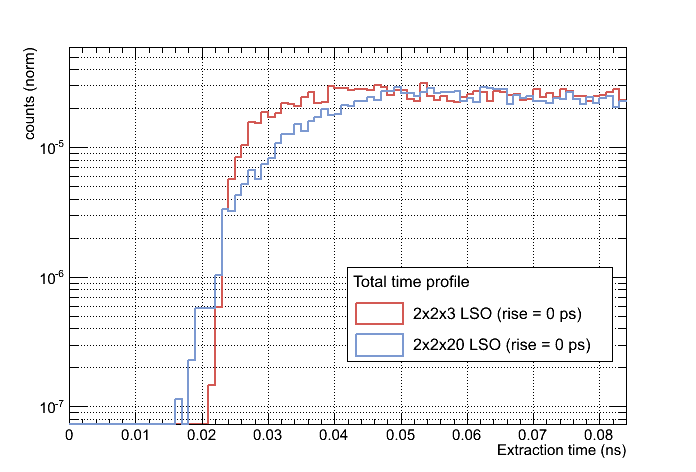
\includegraphics[width=10cm]{../Pictures/Chapter_6/tot_3_20.png}
\end{center}
\caption[Collection scintillation times for LSO naked]{Collection time of scintillation photons produced by a 511 keV $\gamma$ in a LSO crystal. Curves of a 2x2x3 mm$^{3}$ LSO and a 2x2x20 mm$^{3}$ sample with zero rise time are shown.}
\label{fig:scint_3_20}
\end{figure}
It is finally worth to add that collection times are usually translated into time stamps. In order to extract these time stamps, the photo detector and electronics noise add a non-negligible jitter, influenced mainly by the single photon time resolution (SPTR) of the detector itself. This contributes to the smearing of the pulse measured, and thus requires de-convolution routines to extract the time constants we are interested in. As an example consider the kinetics of figure \ref{fig:smear_tot}. Two 2x2x3 mm$^{3}$ LSO crystals are simulated with different rise times, namely 0 ps and 100 ps. In this case a Gaussian smearing was added to the signal, considering a $\sigma _{SPTR}$ of 60 ps. The two curves are barely distinguishable as the SPTR is of the order of magnitude of the rise time and thus tends to wash out the rising profile.   

\begin{figure}[htbp]
\begin{center}
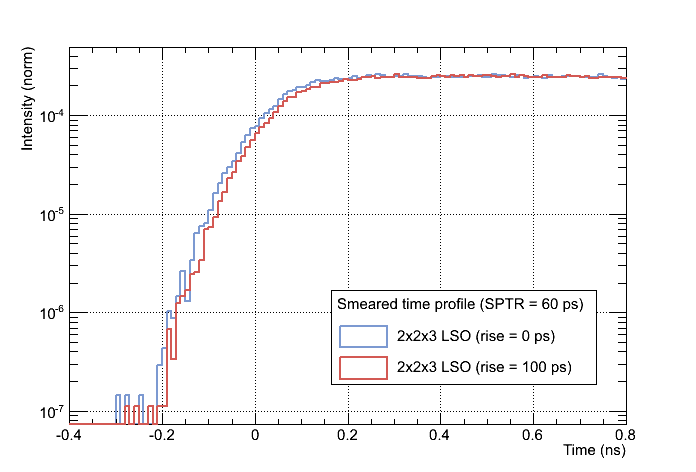
\includegraphics[width=10cm]{../Pictures/Chapter_6/smear_profile.png}
\end{center}
\caption[Collection scintillation times for LSO naked with SPTR smearing]{Collection time of scintillation photons produced by a 511 keV $\gamma$ in a LSO crystal with smearing ($\sigma _{SPTR} = 60 ps$). Curves of 2x2x3 mm$^{3}$ samples with zero  and 100 ps rise time are shown.}
\label{fig:smear_tot}
\end{figure}
\newpage
\subsection{Extraction of time constants}
At this point it is natural to analyse the impact of the elements previously discussed on extracted time constants.
In fact, production stage, transportation stage, Cerenkov photons and resolution smearing all contribute to an effective rise time which will be different than the intrinsic rise time of the relaxation scheme. 
The data analysis approach we chosen is strongly model dependent since the processes just quoted happen on a time scale that is not accessible by our instrumentation. This means that the curve measured will be deconvolved from a measured IRF and the model chosen will be a multi exponential. As a consequence the value extracted for rise time is itself a convolution of different effects.
As will be shown in the next chapter it is possible to disentangle the processes concurring to the formation of the signal using different experimental approaches, in terms of energy excitation, geometry, and surface conditions of the sample measured.

The simulation stage can give already important information for what concerns expectations on the parameters. As an example we considered the output of our simulations, namely scintillation time profiles with and without Cerenkov production, for samples of different aspect ratio and different surface condition. These curves are then smeared by a resolution effect comparable to experimental values we have to deal with ($\sigma _{SPTR}$ = 70 ps) and the rise constant is extracted with the iterative re-convolution routine. It is possible to infer the quantitative influence of collection time RMS on the extracted rise time. In this case the IRF simulated is a simple Gaussian, so we can extend the fit over the entire range without any bias. The decay extracted is 40 ns in every case.

In figure \ref{fig:rise_no_cer} two graphs are reported. LSO samples of extraction face of 2x2 mm$^{2}$ and length of 3, 5, 10 and 20 mm are simulated in two different configurations: 0 ps and 100 ps rise time without Cerenkov production.
In the first case we can see the effect of transportation alone on the rise time extracted, and as expected it increases as the dimension of the crystal increases.
This happens as well in the case of 100 ps rise time, and the transportation phase leads to fit of slower rise times.
% un fit con e senza wrapping
\begin{figure}[htbp]
\begin{center}
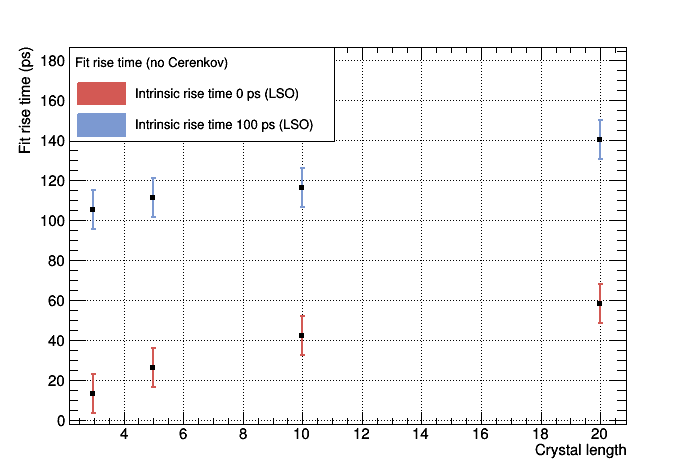
\includegraphics[width=10cm]{../Pictures/Chapter_6/file_without_cer.png}
\end{center}
\caption[Extracted rise time for 0 and 100 ps intrinsic rise time]{Fit rise time for LSO samples of extraction face of 2x2 mm$^{2}$ and length of 3, 5, 10 and 20 mm. Scintillation is produced with 0 ps and 100 ps rise time respectively without Cerenkov production}
\label{fig:rise_no_cer}
\end{figure}
If we add Cerenkov production, the extracted rise times get even slower, as shown in figure \ref{fig:rise_cer} for the case of LSO crystals of different length and intrinsic rise time of 100 ps.
\begin{figure}[htbp]
\begin{center}
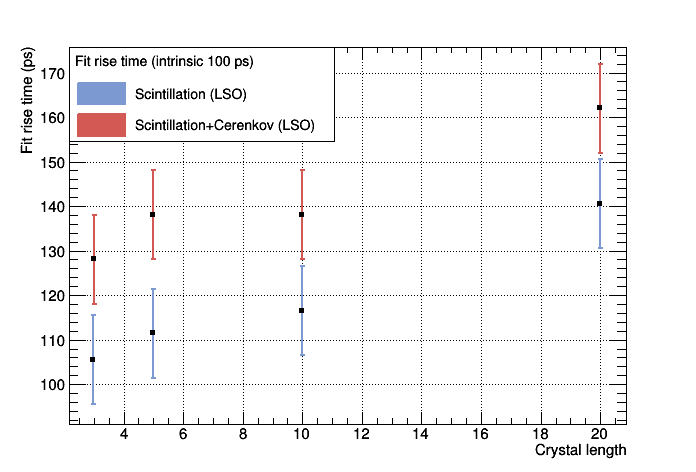
\includegraphics[width=10cm]{../Pictures/Chapter_6/rise_with_cer.png}
\end{center}
\caption[Extracted rise time for scintillation and Cerenkov production]{Fit rise time for LSO samples of extraction face of 2x2 mm$^{2}$ and length of 3, 5, 10 and 20 mm. Scintillation is produced with 100 ps rise time respectively with and without Cerenkov production}
\label{fig:rise_cer}
\end{figure}
A third situation to consider is the interaction at boundaries. If we model Teflon wrapping as completely diffusive, as in the previous section, it is possible to couple out more photons than in a naked configuration. As already shown this increases the RMS in time of the photons extracted. An example is shown in figure \ref{fig:matlab_teflon} and \ref{fig:matlab_no_teflon} where a 0 ps 2x2x5 mm$^{3}$ LSO is simulated with and without Teflon wrapping. In the case of Teflon wrapping the fit rise time is 78 ps and in the case of a naked crystal, as already seen in this section, 25 ps. On the top of each figure, the deviance residuals obtained for likelihood estimation are reported, to graphically show large bias in the fit data if present. This residuals are defined as
\begin{equation}
R_{i} = \sqrt{2\left[ c_{i}\log{\frac{c_{i}}{g_{i}}-c_{i}+g_{i}} \right]}sign\left[ c_{i}-g{i} \right]
\end{equation}
and $c_{i}$ and $g_{i}$ are respectively the counts and the model expectations in channel i.

\begin{figure}[htbp]
\begin{center}
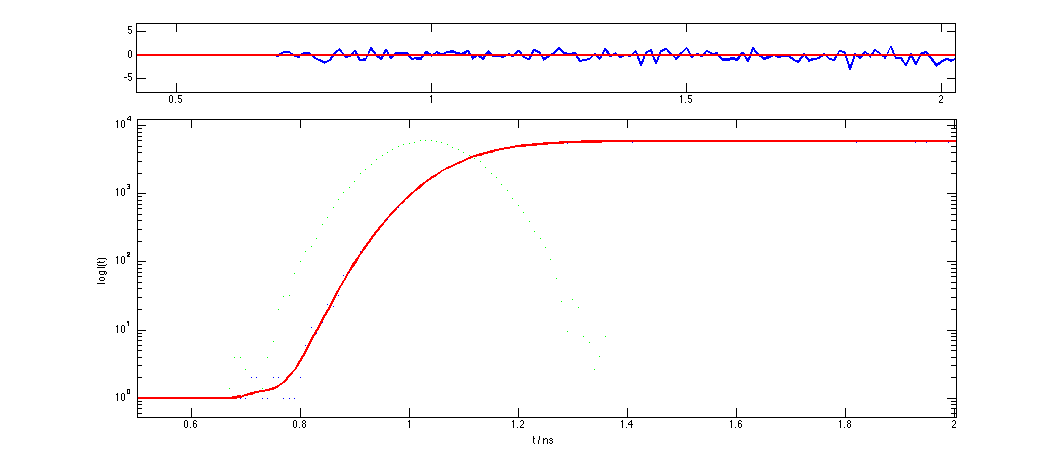
\includegraphics[width=10cm]{../Pictures/Chapter_6/matlab_teflon.png}
\end{center}
\caption[Likelihood fit for LSO naked]{Likelihood fit for 2x2x5 mm$^{3}$ LSO crystal with 100 ns rise time for a 511 KeV $\gamma$ interaction in a naked configuration. The likelihood residuals are shown.}
\label{fig:matlab_teflon}
\end{figure}

\begin{figure}[htbp]
\begin{center}
\includegraphics[width=10cm]{../Pictures/Chapter_6/matlab_no_teflon.png}
\end{center}
\caption[Likelihood fit for LSO Teflon wrapped]{Likelihood fit for 2x2x5 mm$^{3}$ LSO crystal with 100 ns rise time for a 511 KeV $\gamma$ interaction in a Teflon wrapped configuration. The likelihood residuals are shown.}
\label{fig:matlab_no_teflon}
\end{figure}